\begingroup
\def\bone{{1}}
\def\Bepsilon{\mbox{$\epsilon$}}
\def\Bvarphi{\mbox{$\varphi$}}
\def\bB{\mbox{$ B$}}
\def\bC{\mbox{$ C$}}
\def\bE{\mbox{$ E$}}
\def\bF{\mbox{$ F$}}
\def\bN{\mbox{$ N$}}
\def\bP{\mbox{$ P$}}
\def\bS{\mbox{$ S$}}
\def\bT{\mbox{$ T$}}
\def\bX{\mbox{$ X$}}
\def\ba{\mbox{$ a$}}
\def\bb{\mbox{$ b$}}
\def\be{\mbox{$ e$}}
\def\bg{\mbox{$ g$}}
\def\br{\mbox{$ r$}}
\def\bu{\mbox{$ u$}}
\def\bv{\mbox{$ v$}}
\def\bw{\mbox{$ w$}}
\def\twist{CBC.Twist}

\fenicschapter{A computational framework for nonlinear elasticity}
              {A computational framework for \\ nonlinear elasticity}
              {A computational framework for nonlinear elasticity}
              {Harish Narayanan}
              {narayanan}

\index{solid mechanics}
\index{nonlinear elasticity}
\index{elasticity}
\index{hyperelasticity}
\index{CBC.Solve}
\index{CBC.Twist}

Nonlinear elasticity theory plays a fundamental role in modeling the
mechanical response of many polymeric and biological materials. Such
materials are capable of undergoing finite deformation, and their
material response is often characterized by complex, nonlinear
constitutive relationships. (See, for example, \citet{Holzapfel2000}
and \citet{TruesdellNoll1965} and the references within for several
examples.) Because of these difficulties, predicting the response of
arbitrary structures composed of such materials to arbitrary loads
requires numerical computation, usually based on the finite element
method. The steps involved in the construction of the required finite
element algorithms are classical and straightforward in principle, but
their application to non-trivial material models are typically tedious
and error-prone. Our recent work on an automated computational
framework for nonlinear elasticity, \twist, is an attempt to alleviate
this problem.

The focus of this chapter will be to describe the design and
implementation of \twist, as well as providing examples of its
use. The goal is to allow researchers to easily pose and solve
problems in nonlinear elasticity in a straightforward manner, so that
they may focus on higher-level modeling questions without being
hindered by specific implementation issues.

What follows is the proposed outline for the chapter.

The chapter begins with a summary of some key results from classical
nonlinear elasticity theory. This discussion is used to motivate the
design of \twist, which is a DOLFIN \citep{LoggWells2010} module
written in UFL syntax \citep{AlnaesLogg2009} that closely resembles
how the theory is written down on paper. In particular, we will see
how one can easily pose sophisticated material models purely at the
level of specifying a strain energy function. The discourse will then
turn to the primary equation of interest: the balance of linear
momentum of a body posed in the reference configuration. A finite
element scheme for this equation will then be presented, pointing out
how \twist{} leverages the automatic linearization capabilities of UFL
to implement this scheme in a manner that is independent of the
specific material model. The time-stepping schemes that \twist{}
implements will also be discussed. With this in place, we turn to
increasingly complex examples to see how initial- boundary-value
problems in nonlinear elasticity can be posed and solved in \twist{}
using only a few lines of high-level code. The chapter concludes with
some remarks on how one can obtain \twist, along with ideas for its
extension.

\section{Brief overview of nonlinear elasticity theory}

The goal of this section is to present an overview of the mathematical
theory of nonlinear elasticity, which plays an important role in the
design of \twist. Readers interested in a more comprehensive treatment
of the subject are referred to, for example, the classical treatises
of \citet{TruesdellToupin1960} and \citet{TruesdellNoll1965}, or more
modern works such as \citet{Gurtin1981}, \citet{Ogden1997} and
\citet{Holzapfel2000}.

\subsection{Posing the question we aim to answer}

The theory begins by idealizing the elastic body of interest as an open
subset of $\mathbb{R}^{2, 3}$ with a piecewise smooth boundary. At a
{\em reference} placement of the body, $\Omega$, points in the body
are identified by their reference positions, $\bX \in \Omega$. The
treatment presented in this chapter is posed in terms of fields which
are parametrized by reference positions. This is commonly termed the
{\em material} or {\em Lagrangian} description.

In its most basic terms, the {\em deformation} of the body over time
$t \in [0, T]$ is a sufficiently smooth bijective map $\Bvarphi:
\overline{\Omega} \times [0,T] \rightarrow \mathbb{R}^{2, 3}$, where
$\overline{\Omega} :=\ \overline{\Omega\cup\partial\Omega}$ and
$\partial\Omega$ is the boundary of $\Omega$. The restrictions on the
map ensure that the motion it describes is physical and within the
range of applicability of the theory (e.g., disallowing the
interpenetration of matter or the formation of cracks). From this map,
we can construct the {\em displacement field},
%%
\begin{equation}
  \bu(\bX, t) = \Bvarphi(\bX, t) - \bX,
\end{equation}
%%
which represents the displacement of a point in time
relative to its reference position.

With this brief background, we are ready to pose the fundamental
question that \twist{} is designed to answer: Given a body comprised
of a specified elastic material, what is the displacement of the body
when it is subjected to prescribed:
%%
\begin{itemize}
\item {\em Body forces:} These include forces such as the self-weight
  of a body, forces on ferromagnetic materials in magnetic fields,
  etc., which act everywhere in the volume of the body. They are
  denoted by the vector field $\bB(\bX, t)$.
\item {\em Traction forces:} This is the force measured per unit
  surface area acting on the {\em Neumann} boundary of the body,
  $\partial\Omega_{\mathrm{N}}$, and denoted by the vector field
  $\bT(\bX, t)$.
\item {\em Displacement boundary conditions:} These are displacement
  fields prescribed on the {\em Dirichlet} boundary of the body,
  $\partial\Omega_{\mathrm{D}}$.
\end{itemize}
%%
It is assumed that $\partial\Omega_{\mathrm{N}}
\cap \partial\Omega_{\mathrm{D}} = \emptyset$ and
$\overline{\partial\Omega_{\mathrm{N}} \cup \partial\Omega_{\mathrm{D}}}
= \partial\Omega$. These details are depicted in
Figure~\ref{fig:narayanan:continuumpotato}.

\begin{figure}
  \centering
  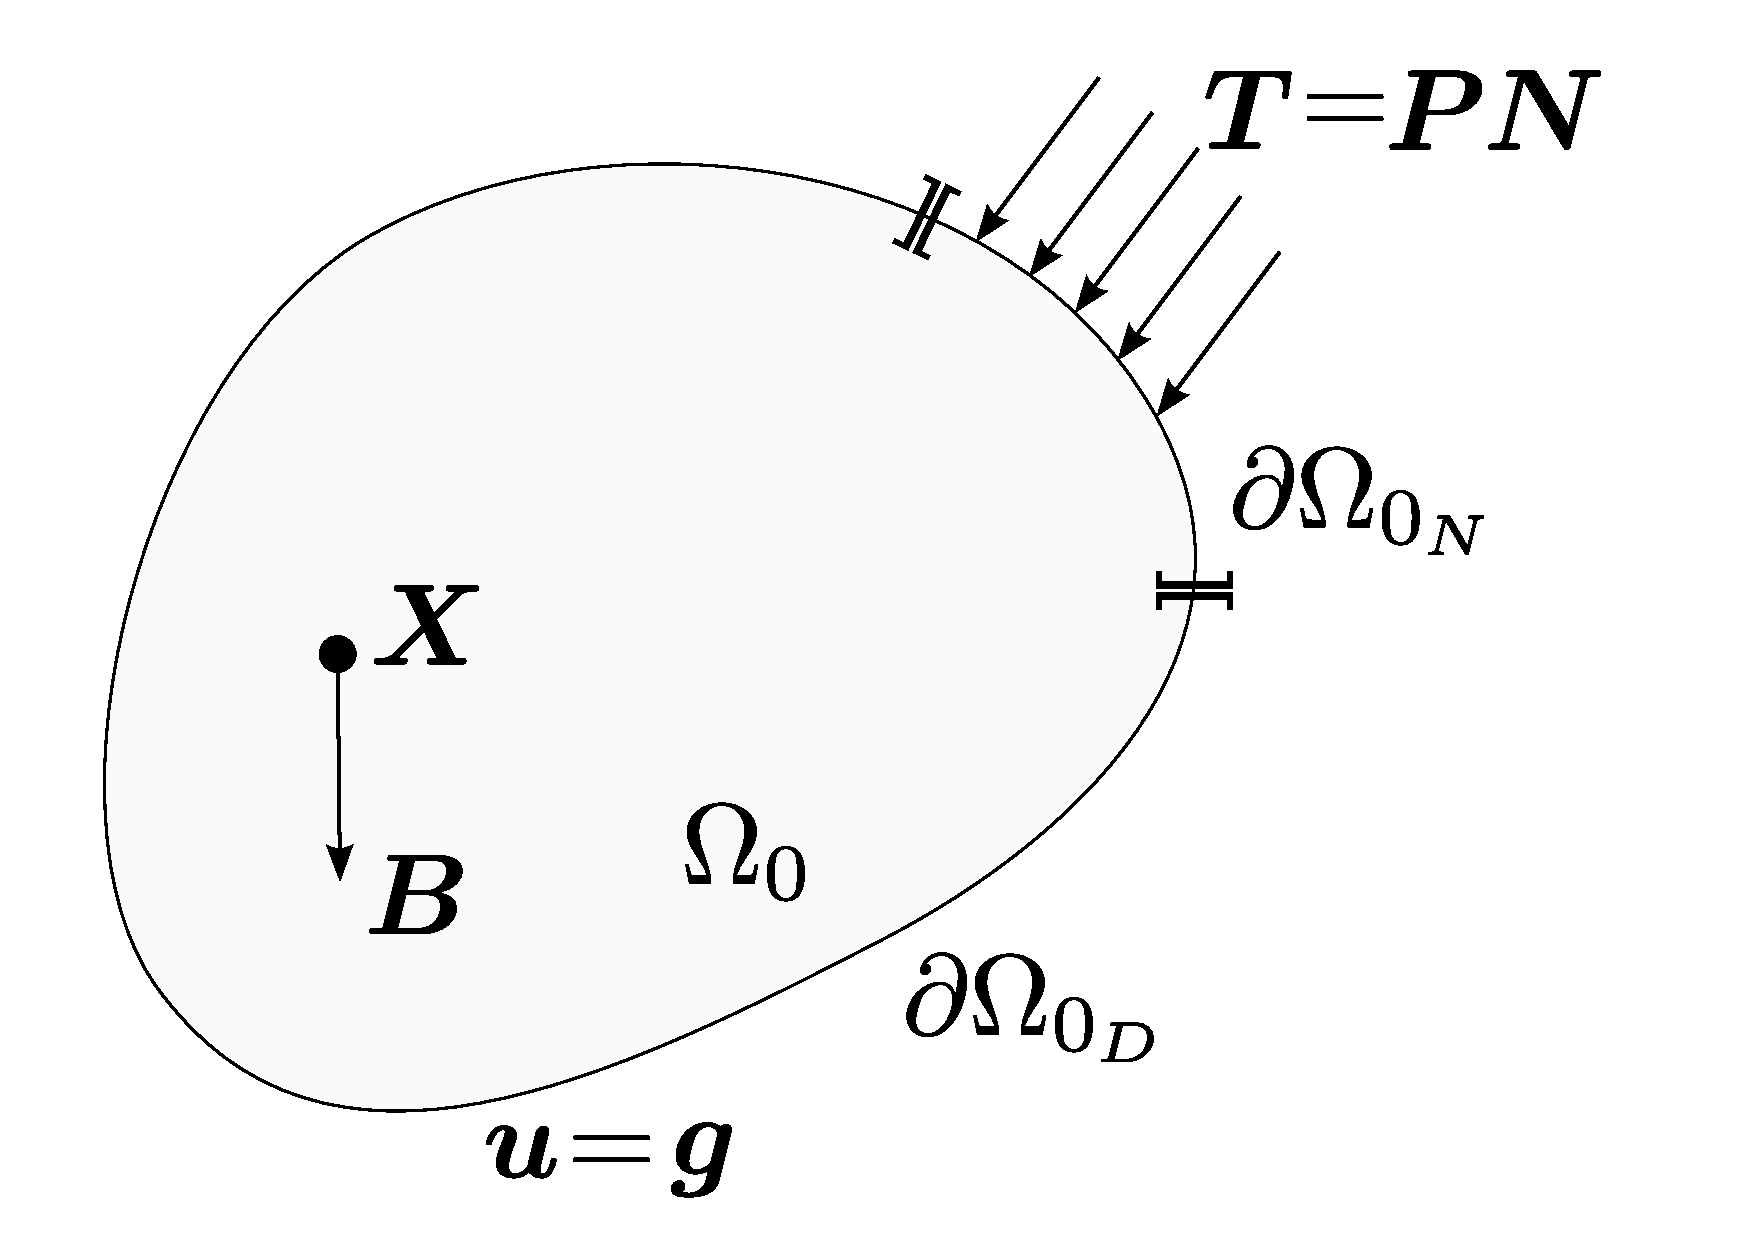
\includegraphics[width=\largefig]{chapters/narayanan/images/pdf/continuumpotato}
  \caption{An elastic body idealized as a continuum, subjected to body
    forces, $\bB$, surface tractions, $\bT$, and prescribed
    displacement boundary conditions.}
    \label{fig:narayanan:continuumpotato}
\end{figure}

\subsection{The basic equation we need to solve}

In order to determine the displacement of an elastic body subjected to
these specified loads and boundary conditions, we turn to a
fundamental law called the {\em balance of linear momentum}. This is a
law which is valid for all materials and must hold for all
time. \twist{} solves the Lagrangian form of this equation, which is
presented below in local form that is pertinent to numerical
implementation by the finite element method:
%%
\begin{equation}
  \rho \frac{\partial^{2} \bu}{\partial t^{2}} = \mathrm{Div}(\bP)
  + \bB\; \mathrm{in}\; \Omega,
  \label{eq:narayanan:balance-of-momentum}
\end{equation}
%%
where $\rho$ is the {\em reference density} of the body, $\bP$ is the
{\em first Piola--Kirchhoff stress tensor}, $\mathrm{Div} (\cdot)$ is
the divergence operator and $\bB$ is the body force per unit
volume. Along with \eqref{eq:narayanan:balance-of-momentum}, we have
initial conditions $\bu(\bX, 0) = \bu_{0}(\bX)$ and
$\frac{\partial\bu}{\partial t}(\bX, 0) = \bv_{0}(\bX)$ in $\Omega$,
and boundary conditions $\bu(\bX, t) = \bg(\bX, t)$ on
$\partial\Omega_{\mathrm{D}}$ and $\bP(\bX, t) \bN(\bX) = \bT(\bX, t)$
on $\partial\Omega_{\mathrm{N}}$. Here, $\bN(X)$ is the outward normal
on the boundary at the point $\bX$.

We focus on the balance of linear momentum because, in a continuous
sense, the other fundamental balance principles that materials must
obey---the balance of mass (continuity equation), balance of angular
momentum and balance of energy---are each trivially
satisfied\footnote{It should be noted that the story is not
  so simple in the context of numerical approximations. For instance,
  when modeling (nearly) incompressible materials, it is well known
  that the ill-conditioned stiffness matrix resulting from the
  conventional Galerkin approximation (discretizing only the
  displacement field) can result in {\em volumetric locking}. One can
  work around this difficulty by resorting to a mixed formulation of
  the Hu--Washizu type~\citep{SimoHughes1998}, but such a formulation
  is beyond the scope of the current chapter. \twist{} can be extended
  to such a formulation, but for now, we circumvent the problem by
  restricting our attention to compressible materials.} in the
Lagrangian description by elastic materials with suitably chosen
stress responses.

\subsection{Accounting for different materials}
\index{material models}

It is important to reiterate that \eqref{eq:narayanan:balance%
-of-momentum} is valid for all materials. In order to differentiate
between different materials and to characterize their specific
mechanical responses, the theory turns to {\em constitutive
relationships}, which are models for describing the real mechanical
behavior of matter. In the case of nonlinear elastic (or {\em
hyperelastic}) materials, this description is usually posed in the
form of a stress-strain relationship through an objective and
frame-indifferent Helmholtz free energy function called the {\em
strain energy function}, $\psi$. This is an energy defined per unit
reference volume and is solely a function of the local {\em strain
measure}. Comprehensive texts on the subject
(e.g. \citet{Holzapfel2000}) cover the motivations for defining
different forms of strain measures, but in this chapter we just
provide the definitions of some of the most common forms. In what
follows, $\mathrm{Grad}(\cdot)$ is the gradient operator, and
$\mathrm{Tr}(\cdot)$ and $\mathrm{Det}(\cdot)$ are the trace and
determinant of $\cdot$, respectively.

\begin{table}
\begin{tabular}{rl}
Infinitesimal strain tensor & $\Bepsilon = \frac{1}{2}
  \left(\mathrm{Grad}(\bu) + \mathrm{Grad}(\bu)^{\mathrm{T}}\right)$
\\
Deformation gradient &  $\bF = \bone + \mathrm{Grad}(\bu)$
\\
Right Cauchy--Green tensor & $\bC = \bF^{\mathrm{T}} \bF$
\\
Green--Lagrange strain tensor & $\bE = \frac{1}{2} \left(\bC -
  \bone\right)$
\\
Left Cauchy--Green tensor & $\bb = \bF \bF^{\mathrm{T}}$
\\
Euler--Almansi strain tensor &  $\be = \frac{1}{2} \left(\bone -
    \bb^{-1}\right)$\\
Volumetric and isochoric\\ decomposition of $\bC$ &  $\bar{\bC} =
  J^{-\frac{2}{3}} \bC$, \quad $J = \mathrm{Det}(\bF)$
\\
Principal invariants of $\bC$ &  $I_{1} =
  \mathrm{Tr}(\bC)$, $I_{2} = \frac{1}{2}\left(I_{1}^{2} -
    \mathrm{Tr}(\bC^{2})\right)$, $I_{3} = \mathrm{Det}(\bC)$
\\
Principal stretches and directions &  $\bC = \sum_{A=1}^{3}
\lambda_{A}^{2} \bN^{A} \otimes \bN^{A}, \quad ||\bN^{A}|| = 1$
\end{tabular}
\caption{Definitions of some common strain measures.}
\label{tab:narayanan:straindefs}
\end{table}

\begin{figure}
\bwfig
\begin{python}
# Deformation gradient
def DeformationGradient(u):
    I = SecondOrderIdentity(u)
    return variable(I + Grad(u))

# Determinant of the deformation gradient
def Jacobian(u):
    F = DeformationGradient(u)
    return variable(det(F))

# Right Cauchy-Green tensor
def RightCauchyGreen(u):
    F = DeformationGradient(u)
    return variable(F.T*F)

# Green-Lagrange strain tensor
def GreenLagrangeStrain(u):
    I = SecondOrderIdentity(u)
    C = RightCauchyGreen(u)
    return variable(0.5*(C - I))

# Invariants of an arbitrary tensor, A
def Invariants(A):
    I1 = tr(A)
    I2 = 0.5*(tr(A)**2 - tr(A*A))
    I3 = det(A)
    return [I1, I2, I3]

# Isochoric part of the deformation gradient
def IsochoricDeformationGradient(u):
    F = DeformationGradient(u)
    J = Jacobian(u)
    return variable(J**(-1.0/3.0)*F)

# Isochoric part of the right Cauchy-Green tensor
def IsochoricRightCauchyGreen(u):
    C = RightCauchyGreen(u)
    J = Jacobian(u)
    return variable(J**(-2.0/3.0)*C)
\end{python}
\caption{Samples of how strain measures are implemented in
  \twist. Notice that the definitions in the implementation closely
  resemble the classical forms introduced in
  Table~\ref{tab:narayanan:straindefs}.}
\label{code:narayanan:kinematics.py}
\end{figure}

In \twist, each of the forms listed in
Table~\ref{tab:narayanan:straindefs} have been implemented in the file
\emp{kinematics.py} in UFL notation that closely resemble their
definitions above. Figure~\ref{code:narayanan:kinematics.py} presents
a section of this file. Notice that it is straightforward to introduce
other custom measures as required.

The stress response of isotropic hyperelastic materials (the class of
materials \twist{} restricts its attention to) can be derived from the
scalar-valued strain energy function. In particular, the tensor known
as the {\em second Piola--Kirchhoff stress tensor} is defined using the
following {\em constitutive relationship}:
%%
\begin{equation}
  \bS = \bF^{-1} \frac{\partial \psi(\bF)}{\partial \bF}.
\end{equation}
%%
The second Piola--Kirchhoff stress tensor is related to the first
Piola--Kirchhoff stress tensor introduced earlier through the relation,
$\bP = \bF \bS$.

As already mentioned, the strain energy function can be posed in
equivalent forms in terms of different strain measures. (Again, the
interested reader is directed to classical texts to motivate this.) In
order to then arrive at the second Piola--Kirchhoff stress tensor, we
turn to the chain rule of differentiation. For example,\enlargethispage{12pt}
%%
\begin{equation}
  \begin{split}
    \bS & = 2 \frac{\partial \psi(\bC)}{\partial \bC} =
    \frac{\partial \psi(\bE)}{\partial \bE}\\
    & = 2\left[\left(\frac{\partial \psi (I_{1}, I_{2},
          I_{3})}{\partial I_{1}} + I_{1} \frac{\partial \psi (I_{1},
          I_{2}, I_{3})}{\partial I_{2}} \right) \bone -
      \frac{\partial \psi (I_{1}, I_{2}, I_{3})}{\partial I_{2}} \bC +
      I_{3} \frac{\partial \psi (I_{1}, I_{2}, I_{3})}{\partial I_{3}}
      \bC^{-1} \right]\\
    & = \sum_{A = 1}^{3} \frac{1}{\lambda_{A}} \frac{\partial
      \psi(\lambda_{1}, \lambda_{2}, \lambda_{3})}{\partial
      \lambda_{A}} \bN^{A}\otimes\bN^{A} = \ldots
  \end{split}
  \label{eq:narayanan:secondpk}
\end{equation}

Using definitions such as the ones explicitly provided in
\eqref{eq:narayanan:secondpk}, \twist{} computes the second
Piola--Kirchhoff stress tensor from the strain energy function by
suitably differentiating it with respect to the appropriate strain
measure. This allows the user to easily specify material models in
terms of each of the strain measures introduced in Table~\ref{tab:%
narayanan:straindefs}. The base class for all material models,
\emp{MaterialModel}, encapsulates this functionality. The relevant
method of this class is provided in Figure~\ref{code:narayanan:%
material_model_base.py}. The implementation relies heavily on the UFL
\emp{diff} operator.

\begin{figure}
\bwfig
\begin{python}
def SecondPiolaKirchhoffStress(self, u):

    ...

    if kinematic_measure == "InfinitesimalStrain":
        epsilon = self.epsilon
        S = diff(psi, epsilon)
    elif kinematic_measure == "RightCauchyGreen":
        C = self.C
        S = 2*diff(psi, C)
    elif kinematic_measure == "GreenLagrangeStrain":
        E = self.E
        S = diff(psi, E)
    elif kinematic_measure == "CauchyGreenInvariants":
        I = self.I; C = self.C
        I1 = self.I1; I2 = self.I2; I3 = self.I3
        gamma1 = diff(psi, I1) + I1*diff(psi, I2)
        gamma2 = -diff(psi, I2)
        gamma3 = I3*diff(psi, I3)
        S = 2*(gamma1*I + gamma2*C + gamma3*inv(C))

    ...
    return S
\end{python}
\caption{Partial listing of the method that suitably computes the
  second Piola--Kirchhoff stress tensor based on the chosen strain
  measure.}
\label{code:narayanan:material_model_base.py}
\end{figure}

The generality of the material model base class allows for the (almost
trivial) specification of a large set of models. To see this in
practice, let us consider two popular material models,
%%
\begin{itemize}
  \item the {\em St.~Venant--Kirchhoff} model: $\psi_{\mathrm{SVK}} =
  \frac{\lambda}{2}\mathrm{Tr}(\bE)^{2} + \mu\mathrm{Tr}(\bE^{2})$, and

  \item the two term {\em Mooney--Rivlin} model: $\psi_{\mathrm{MR}} =
  c_{1} (I_{1} - 3) + c_{2} (I_{2} - 3)$,
\end{itemize}
%%
and see how they can be specified in \twist. The relevant blocks of code
are shown in Figures~\ref{code:narayanan:svk} and \ref{code:narayanan:mr}.
Clearly, the code simply contains the strain energy function
in classical notation, along with some metadata clarifying the number
of material parameters and the strain measure the model relies on. The
file \emp{material\_models.py} contains several other material models,
including {\em linear elasticity, neo Hookean, Isihara, Biderman,} and
{\em Gent--Thomas} that come pre-implemented in \twist. (Refer to the
article by \citet{MarckmannVerron2006} comparing several hyperelastic
models for rubber-like materials for their definitions.) But the
salient point to note here is that it is straightforward to introduce
other additional models, and this is a significant feature of \twist.

\begin{figure}
\bwfig
\begin{python}
class StVenantKirchhoff(MaterialModel)

    def model_info(self):
        self.num_parameters = 2
        self.kinematic_measure = "GreenLagrangeStrain"

    def strain_energy(self, parameters):
        E = self.E
        [mu, lmbda] = parameters
        return lmbda/2*(tr(E)**2) + mu*tr(E*E)
\end{python}
\caption{Definition the strain energy function for a
  St.~Venant--Kirchhoff material.}
\label{code:narayanan:svk}
\end{figure}

\begin{figure}
\bwfig
\begin{python}
class MooneyRivlin(MaterialModel)

    def model_info(self):
        self.num_parameters = 2
        self.kinematic_measure = "CauchyGreenInvariants"

    def strain_energy(self, parameters):
        I1 = self.I1
        I2 = self.I2
        [C1, C2] = parameters
        return C1*(I1 - 3) + C2*(I2 - 3)
\end{python}
\caption{Definition the strain energy function for a two term
  Mooney--Rivlin material.}
\label{code:narayanan:mr}
\end{figure}

\section{Numerical methods and further implementation details}

In the preceding section, we saw the functionality that \twist{}
provided to easily specify material models to suitably characterize
different materials of interest. In this section, we return to the
general form of the balance of linear momentum and look at details of
a finite element formulation and implementation for this equation. For
further details on the treatment that follows, the interested reader
is directed to \citet{SimoHughes1998}.

\subsection{The finite element formulation of the balance of linear
  momentum}

By taking the dot product of \eqref{eq:narayanan:balance-of-momentum}
with a test function $\bv \in \hat{\mathrm{V}}$ and integrating over
the reference domain and time, we have
%%
\begin{equation}
  \int_{0}^{T} \int_{\Omega} \rho \frac{\partial^{2}
    \bu}{\partial t^{2}} \cdot \bv \dx \dt\;
  = \int_{0}^{T}\int_{\Omega} \mathrm{Div}(\bP) \cdot \bv \dx \dt\;
  + \int_{0}^{T} \int_{\Omega} \bB \cdot \bv \dx \dt.
\end{equation}
%%
Noting that the traction vector $\bT = \bP \bN$ on
$\partial\Omega_{\mathrm{N}}$ ($\bN$ being the outward normal on the
boundary) and that by definition $\bv|_{\partial\Omega_{\mathrm{D}}} =
0$, we apply the divergence theorem to arrive at the following weak
form of the balance of linear momentum: \\*
Find $\bu \in \mathrm{V}$, such that $\foralls \bv \in
\hat{\mathrm{V}}$:
%%
\begin{equation}
  \int_{0}^{T} \int_{\Omega} \rho \frac{\partial^{2} \bu}{\partial
    t^{2}} \cdot \bv \dx \dt\; + \int_{0}^{T} \int_{\Omega}
  \bP:\mathrm{Grad}(\bv) \dx \dt\; = \int_{0}^{T} \int_{\Omega} \bB
  \cdot \bv \dx \dt\; + \int_{0}^{T} \int_{\partial\Omega_{\mathrm{N}}}
  \bT \cdot \bv \ds \dt,
\label{eq:narayanan:weakform}
\end{equation}
%%
with initial conditions $\bu(\bX, 0) = \bu_{0}(\bX)$ and
$\frac{\partial\bu}{\partial t}(\bX, 0) = \bv_{0}(\bX)$ in $\Omega$,
and boundary conditions $\bu(\bX, t) = \bg(\bX, t)$ on
$\partial\Omega_{\mathrm{D}}$.

The finite element formulation implemented in \twist{} follows the
Galerkin approximation of the above weak form~\eqref{eq:narayanan:%
weakform}, by looking for solutions in a finite solution space
$\mathrm{V}_{h} \subset \mathrm{V}$ and allowing for test functions in
a finite approximation of the test space $\hat{\mathrm{V}}_{h} \subset
\hat{\mathrm{V}}$.\footnote{We now note an inherent advantage in
  choosing the Lagrangian description in formulating the theory. The
  fact that the integrals in \eqref{eq:narayanan:weakform}, along with
  the various fields and differential operators, are defined over the
  fixed domain $\Omega$ means that one need not be concerned with the
  complexity associated with calculations on a moving computational
  domain when implementing this formulation.}

\vspace*{-3pt}
\subsection{Implementation of the static form}

We consider first the static weak form (dropping the time derivative
term) of the balance of linear momentum which reads\vspace*{-2pt}
%%
\begin{equation}
  \int_{\Omega} \bP:\mathrm{Grad}(\bv) \dx - \int_{\Omega} \bB
  \cdot \bv \dx -  \int_{\partial\Omega_{\mathrm{N}}} \bT \cdot
  \bv \ds = 0.
\label{eq:narayanan:staticweakform}\vspace*{-2pt}
\end{equation}
%%
Since \twist{} provides the necessary functionality to easily compute
the first Piola--Kirchhoff stress tensor, $\bP$, given a displacement
field, $\bu$, for arbitrary material models, \eqref{eq:narayanan:%
staticweakform} is just a nonlinear functional in terms of $\bu$. The
automatic differentiation capabilities of UFL\footnote{An earlier
  chapter on UFL~(\ref{chap:alnes-1}) provides a detailed look at the
  capabilities of UFL, as well as insights into how it achieves its
  functionality. Even so, we note the following differentiation
  capabilities of UFL because of their pivotal relevance to this work:
%%
  \begin{itemize}
  \item Computing spatial derivatives of fields, which allows for the
    construction of differential operators such as such as
    $\mathrm{Grad(\cdot)}$ or $\mathrm{Div(\cdot)}$:\\
    \texttt{df\_i = Dx(f, i)}
  \item Differentiating arbitrary expressions with respect to variables
    they are functions of:\\
    \texttt{g = variable(cos(cell.x[0]))}\\
    \texttt{f = exp(g**2)}\\
    \texttt{h = diff(f, g)}
  \item Differentiating forms with respect to coefficients of a discrete
    function, allowing for automatic linearizations of nonlinear
    variational forms:\\
    \texttt{a = derivative(L, w, u)}
  \end{itemize}} make this nonlinear form straightforward to
implement, as evidenced by the code listing in Figure~\ref{code:%
narayanan:staticmomentumsolver}.\enlargethispage{6pt}

This listing provides the relevant section of the static balance of
linear momentum solver class, \emp{StaticMomentumBalanceSolver}. The
class draws information about the problem (mesh, loading, boundary
conditions and form of the stress equation derived from the material
model) from the user-specified problem class,\footnote{Details of how
the user can specify problem details are covered in the following
section containing examples of \twist{} usage.} and solves the
nonlinear momentum balance equation using a Newton solver.

\begin{figure}[!t]
\bwfig
\begin{python}
# Get the problem mesh
mesh = problem.mesh()

# Define the function space
vector = VectorFunctionSpace(mesh, "Lagrange", 1)

# Test and trial functions
v = TestFunction(vector)
u = Function(vector)
du = TrialFunction(vector)

# Get forces and boundary conditions
B = problem.body_force()
PN = problem.surface_traction()
bcu = problem.boundary_conditions()

# First Piola-Kirchhoff stress tensor based on
# the material model
P = problem.first_pk_stress(u)

# The variational form corresponding to static
# hyperelasticity
L = inner(P, Grad(v))*dx - inner(B, v)*dx - inner(PN, v)*ds
a = derivative(L, u, du)

# Setup and solve problem
problem = NonlinearVariationalProblem(L, u, bcu, a)
solver = NonlinearVariationalSolver(problem)
solver.solve()
\end{python}
\caption{The relevant section of the class
\emp{StaticMomentumBalanceSolver}, the solver for the static balance of
linear momentum.}
\label{code:narayanan:staticmomentumsolver}
\end{figure}

\vspace*{-3pt}
\subsection{Time-stepping algorithms}
\index{time integration}

\twist{} implements two time integration algorithms to solve the weak
form of the fully dynamic balance of linear momentum
\eqref{eq:narayanan:weakform}. The first of these is the
so-called CG$_{1}$ method \citep{ErikssonEstepHansboEtAl1996}. In order
to derive this method, \eqref{eq:narayanan:weakform}, which is
a second order differential equation in time, is rewritten as a system
of first order equations. We do this by introducing an additional
velocity variable, $\bw = \frac{\partial \bu}{\partial t}$. Thus, the
weak form now reads:

\noindent Find ($\bu, \bw) \in \mathrm{V}$, such that $\foralls (\bv,
\br) \in \hat{\mathrm{V}}$:
%%
\begin{equation}
  \begin{split}
    \int_{0}^{T} \int_{\Omega} \rho \frac{\partial \bw}{\partial t}
    \cdot \bv \dx \dt\; + \int_{0}^{T} \int_{\Omega}
    \bP:\mathrm{Grad}(\bv) \dx \dt\;
    &= \int_{0}^{T} \int_{\Omega} \bB \cdot \bv \dx \dt\; +
    \int_{0}^{T} \int_{\partial\Omega_{\mathrm{N}}} \bT \cdot \bv \ds
    \dt, \; \mathrm{and}\\
    \int_{0}^{T} \int_{\Omega} \frac{\partial \bu}{\partial t} \cdot
    \br \dx \dt\;
    &= \int_{0}^{T} \int_{\Omega} \bw \cdot \br \dx \dt.
  \end{split}
\label{eq:narayanan:cg1weakform}
\end{equation}
%%
with initial conditions $\bu(\bX, 0) = \bu_{0}(\bX)$ and $w(\bX, 0)
= \bv_{0}(\bX)$ in $\Omega$, and boundary conditions $\bu(\bX, t) =
\bg(\bX, t)$ on $\partial\Omega_{\mathrm{D}}$.

We now assume that the finite element approximation space
$\mathrm{V}_{h}$ is CG$_{1}$ (continuous and piecewise linear in time),
and $\hat{\mathrm{V}}_{h}$ is DG$_{0}$ (discontinuous and piecewise
constant in time). With these assumptions, we arrive at the following
scheme:
%%
\begin{equation}
  \begin{split}
    \int_{\Omega} \rho \frac{\left(\bw_{n+1} - \bw_{n}\right)}{\Delta
      t} \cdot \bv \dx\; + \int_{\Omega}
    \bP(\bu_{\mathrm{mid}}):\mathrm{Grad}(\bv) \dx\;
    &=  \int_{\Omega} \bB \cdot \bv \dx\;
    +  \int_{\partial\Omega_{\mathrm{N}}} \bT \cdot \bv \ds,
    \; \mathrm{and}\\
    \int_{\Omega} \frac{\left(\bu_{n+1} - \bu_{n}\right)}{\Delta t}
    \cdot \br \dx\;
    &=  \int_{\Omega} \bw_{\mathrm{mid}} \cdot \br \dx,
\end{split}
\label{eq:narayanan:cg1weakformapprox}
\end{equation}
%%
where $(\cdot)_{n}$ and $(\cdot)_{n+1}$ are the values of a
quantity at the current and subsequent time-step, respectively, and
$(\cdot)_{\mathrm{mid}} = \frac{(\cdot)_{n} +
  (\cdot)_{n+1}}{2}$. A section of the CG$_{1}$ linear momentum balance
solver class is presented in Figure~\ref{code:narayanan:cg1}. The
code closely mirrors the scheme defined in
\eqref{eq:narayanan:cg1weakformapprox}, and results in a mixed system
that is solved for using a Newton scheme.

\begin{figure}
\bwfig
\begin{python}
class CG1MomentumBalanceSolver(CBCSolver):

    # Define function spaces
    vector = VectorFunctionSpace(mesh, "Lagrange", 1)
    mixed_element = MixedFunctionSpace([vector,
                                        vector])
    V = TestFunction(mixed_element)
    dU = TrialFunction(mixed_element)
    U = Function(mixed_element)
    U0 = Function(mixed_element)

    # Get initial conditions, boundary conditions
    # and body forces
    ...

    # Functions
    v, r = split(V)
    u, w = split(U)
    u0, w0 = split(U0)

    # Evaluate displacements and velocities at
    # mid points
    u_mid = 0.5*(u0 + u)
    w_mid = 0.5*(w0 + w)

    # Get reference density
    rho = problem.reference_density()

    # Piola-Kirchhoff stress tensor based on the
    # material model
    P = problem.first_pk_stress(u_mid)

    # The variational form corresponding to
    # dynamic hyperelasticity
    L = rho*inner(w - w0, v)*dx \
        + dt*inner(P, grad(v))*dx \
        - dt*inner(B, v)*dx\
        + inner(u - u0, r)*dx \
        - dt*inner(w_mid, r)*dx

    # Add contributions to the form from the
    # Neumann boundary conditions
    ...

    a = derivative(L, U, dU)
\end{python}
\caption{Relevant portion of the dynamic balance of linear momentum
  solver using the CG$_{1}$ time-stepping scheme.}
\label{code:narayanan:cg1}
\end{figure}

The CG$_{1}$ scheme defined in \eqref{eq:narayanan:cg1weak%
formapprox} is straightforward to derive and implement, and it is
second order accurate and energy conserving.\footnote{This is
  demonstrated in Figure~\ref{fig:narayanan:energies} as part of the
  second example calculation.}  But it should also be noted that the mixed
system that results from the formulation is computationally expensive
and memory intensive, as the number of variables being solved for have
doubled due to the introduction of the velocity variable.

\twist{} also provides a standard implementation of a finite
difference time-stepping algorithm that is commonly used in the
computational mechanics community: the Hilber--Hughes--Taylor (HHT)
method \citep{HilberHughesTaylor1977}. The stability and dissipative
properties of this method in the case of linear problems have been
thoroughly discussed in \citet{Hughes1987}. In particular, the method
contains three parameters $\alpha$, $\beta$ and $\gamma$ which control
the accuracy, stability and numerical dissipation of the scheme. The
default values for these parameters chosen in \twist{} ($\alpha = 1$,
$\beta = \frac{1}{4}$ and $\gamma = \frac{1}{2}$) ensure that the
method is second order accurate, stable for linear problems and
introduces no numerical dissipation.

The method is briefly sketched below. For further details about the scheme
itself, or its implementation in \twist, the interested reader is directed
to the previously mentioned papers, and the \emp{MomentumBalanceSolver}
class in the file \emp{solution\_algorithms.py}.

Given initial conditions $\bu(\bX, 0) = \bu_{0}(\bX)$ and
$\frac{\partial\bu}{\partial t}(\bX, 0) = \bv_{0}(\bX)$, we can
compute the initial acceleration, $\ba_{0}$, from the weak form:
%%
\begin{equation}
  \int_{\Omega} \rho a_{0} \cdot \bv \dx\; +  \int_{\Omega}
  \bP(u_{0}):\mathrm{Grad}(\bv) \dx\; - \int_{\Omega} \bB(X, 0)
  \cdot \bv \dx\; -  \int_{\partial\Omega_{\mathrm{N}}}
  \bT(X, 0) \cdot \bv \ds = 0.
\end{equation}
%%
This provides the complete initial state ($\bu_{0}, \bv_{0}, \ba_{0}$)
of the body. Now, given the solution at time step $n$, the HHT formulae
advance the solution to step $n+1$ as follows. First, we note the
following definitions:
%%
\begin{equation}
  \begin{split}
    \bu_{n+1} & = \bu_{n} + \Delta t \bv_{n} + \Delta t^{2} \left[
      \left(\frac{1}{2} - \beta \right) \ba_{n} + \beta \ba_{n+1}
    \right]\\
    \bv_{n+1} & = \bv_{n} + \Delta t \left[ (1-\gamma) \ba_{n} +
      \gamma \ba_{n+1} \right]\\
    \bu_{n+\alpha} & = (1 - \alpha) \bu_{n} + \alpha \bu_{n+1}\\
    \bv_{n+\alpha} & = (1 - \alpha) \bv_{n} + \alpha \bv_{n+1}\\
    t_{n+\alpha} &= (1 - \alpha) t_{n} + \alpha t_{n + 1}
\end{split}
\label{eq:narayanan:hhtdefs}
\end{equation}
%%
Inserting the definitions in \eqref{eq:narayanan:hhtdefs}
into the following form of the balance of linear momentum,
%%
\begin{equation}
   \int_{\Omega} \rho a_{n+1} \cdot \bv \dx\; + \int_{\Omega} \bP(u_{n
     + \alpha}):\mathrm{Grad}(\bv) \dx\; - \int_{\Omega} \bB(X, t_{n +
     \alpha}) \cdot \bv \dx\; - \int_{\partial\Omega_{\mathrm{N}}}
   \bT(X, t_{n + \alpha}) \cdot \bv \ds = 0,
\label{eq:narayanan:newaccn}
\end{equation}
%%
we can solve for the for the only unknown variable, the acceleration
at the next step, $\ba_{n+1}$. The acceleration solution to
\eqref{eq:narayanan:newaccn} is then used in the definitions%
~\eqref{eq:narayanan:hhtdefs} to update to new displacement and
velocity values, and the problem is stepped through time.

We close this subsection on time-stepping algorithms with one usage
detail pertaining to \twist. By default, when solving a dynamics
problem, \twist{} assumes that the user wants to use the HHT
method. In case one wants to override this behavior, they can do so by
returning \emp{"CG(1)"} in the \emp{time\_stepping} method while
specifying the problem. Figure~\ref{code:narayanan:dynamicrelease} is
an example showing this.

\section{Examples of \twist{} usage}
\index{CBC.Twist}

The algorithms discussed thus far serve primarily to explain the
computational framework's inner working, and are not at the level at
which the user usually interacts with \twist{} (unless they are
interested in extending it). In practice, the functionality of
\twist{} is exposed to the user through two primary problem definition
classes: \emp{StaticHyperelasticity} and \emp{Hyperelasticity}. These
classes reside in \emp{problem\_definitions.py}, and contain numerous
methods for defining aspects of the nonlinear elasticity problem. As
their names suggest, these are respectively used to describe static or
dynamic problems in nonlinear elasticity.

Over the course of the following examples, we will see how various
problems can be defined in \twist{} by suitably deriving from these
problem classes and overloading relevant methods.\footnote{The
examples presented in this chapter, along with a few others, reside in
the \emp{demos/twist/} folder in \twist's source repository. They can
be run by navigating to this folder and typing \emp{python
demo\_name.py} on the command-line.} We will also see some results
from these calculations. The information defined in the problem
classes are internally transferred to the solvers described earlier to
actually solve the problem.

\subsection{The static twisting of a hyperelastic cube}

The first problem we are interested in is the twisting of a unit
hyperelastic cube (1~m$^3$). The cube is assumed to be made out of a
St.~Venant--Kirchhoff material with Lam\'e's parameters $\mu =
3.8461$~N/m$^2$ and a spatially varying $\lambda = 5.8 x_{1} + 5.7 (1
- x_{1})$~N/m$^2$. Here, $x_{1}$ is the first coordinate of the
reference position, $\bX$.\footnote{The numerical parameters in this
  chapter have been arbitrarily chosen for illustration of the
  framework's use. They do not necessarily correspond to a real
  material.} In order to twist the cube, the face $x_{1} = 0$ is held
fixed and the opposite face $x_{1} = 1$ is rotated 60 degrees using
the Dirichlet condition defined in
Figure~\ref{code:narayanan:statictwist}.

\begin{figure}
\bwfig
  \centering
  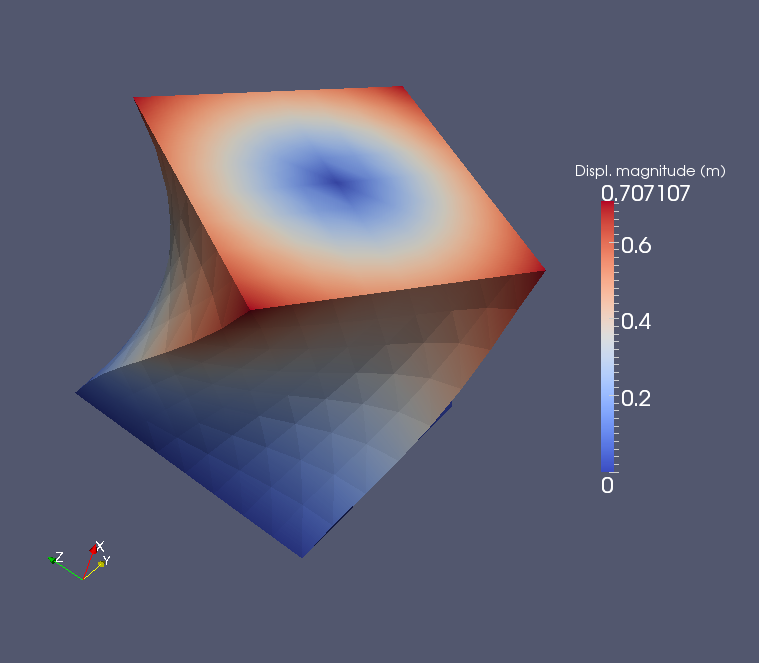
\includegraphics[width=0.6\textwidth]{chapters/narayanan/images/png/twistedcube.png}
  \caption{A hyperelastic cube twisted by 60 degrees.}
    \label{fig:narayanan:twistedcube}
\end{figure}

Before getting to the actual specification of the problem in code, we
need to import \twist's functionality:
%%
\begin{python}
from cbc.twist import *
\end{python}
%%
The problem is completely specified by defining relevant methods in
the user-created class \emp{Twist} (see
Figure~\ref{code:narayanan:statictwist}), which derives from the base
class \emp{StaticHyperelasticity}. \twist{} only requires relevant
methods to be provided, and for the current problem, this includes
those that define the computational domain, Dirichlet boundary
conditions and material model. The methods are fairly
self-explanatory, but the following points are to be noted. Firstly,
\twist{} supports spatially-varying material parameters. Secondly,
Dirichlet boundary conditions are posed in two parts: the conditions
themselves, and the corresponding boundaries along which they act.

\begin{figure}
\bwfig
\begin{python}
class Twist(StaticHyperelasticity):

    def mesh(self):
        n = 8
        return UnitCube(n, n, n)

    def dirichlet_conditions(self):
        clamp = Expression(("0.0", "0.0", "0.0"))
        twist = Expression(("0.0",
        "y0+(x[1]-y0)*cos(theta)-(x[2]-z0)*sin(theta)-x[1]",
        "z0+(x[1]-y0)*sin(theta)+(x[2]-z0)*cos(theta)-x[2]"),
        y0=0.5, z0=0.5, theta=pi/3)
        return [clamp, twist]

    def dirichlet_boundaries(self):
        return ["x[0] == 0.0", "x[0] == 1.0"]

    def material_model(self):
        mu    = 3.8461
        lmbda = Expression("x[0]*5.8+(1-x[0])*5.7")

        material = StVenantKirchhoff([mu, lmbda])
        return material

    def __str__(self):
        return "A cube twisted by 60 degrees"
\end{python}
\caption{Problem definition: The static twisting of a hyperelastic
  cube.}
\label{code:narayanan:statictwist}
\end{figure}

In order to solve this problem, an instance of the \emp{Twist} class
is created and its \emp{solve} method is called (see
Figure~\ref{code:narayanan:solveproblem}). This triggers a Newton
solve which exhibits quadratic convergence (see
Table~\ref{tab:narayanan:residualnorms}) and results in the
displacement field shown in
Figure~\ref{fig:narayanan:twistedcube}.

\begin{figure}
\bwfig
\begin{python}
twist = Twist()
u = twist.solve()
\end{python}
\caption{Solving the posed problem.}
\label{code:narayanan:solveproblem}
\end{figure}

\begin{table}
  \centering
    \begin{tabular}{cc}
      \toprule
      Iteration & Relative Residual Norm \\
      \midrule
      1 & 5.835e-01\\
      2 & 1.535e-01\\
      3 & 3.640e-02\\
      4 & 1.004e-02\\
      5 & 1.117e-03\\
      6 & 1.996e-05\\
      7 & 9.935e-09\\
      8 & 3.844e-15\\
      \bottomrule
    \end{tabular}
    \caption{Quadratic convergence of the Newton method used to solve
      the hyperelasticity problem. It is interesting to note that this
      convergence is obtained even though the 60 degree twist
      condition was imposed in a single step.}
    \label{tab:narayanan:residualnorms}
\end{table}

\subsection{The dynamic release of a twisted cube}

In this problem, we release a unit cube (1~m$^3$) that has previously
been twisted. The initial twist was precomputed in a separate
calculation involving a traction force on the top surface and the
resulting displacement field was stored in the file {\tt
twisty.txt}. The release calculation loads this solution as the
initial displacement. It fixes the cube (made of a
St.~Venant--Kirchhoff material with Lam\'e's parameters $\mu =
3.8461$~N/m$^2$ and $\lambda = 5.76$~N/m$^2$) on the bottom surface,
and tracks the motion of the cube over 2~s.

The problem is specified in the user-created class \emp{Release},
which derives from \emp{Hyperelasticity}. This example is similar to
the previous one, except that since it is a dynamic calculation, it also
provides initial conditions, a reference density and information about
time-stepping. Again, the methods listed in
Figure~\ref{code:narayanan:dynamicrelease} are straightforward, and
the only additional point to note is that \twist{} provides some
convenience utilities to simplify the specification of the
problem. For example, one can load initial conditions directly from
files, and it allows for the specification of boundaries purely as
conditional strings.

\begin{figure}
\bwfig
\begin{python}
class Release(Hyperelasticity):

    def mesh(self):
        n = 8
        return UnitCube(n, n, n)

    def end_time(self):
        return 2.0

    def time_step(self):
        return 2.e-3

    def time_stepping(self):
        return "CG(1)"

    def reference_density(self):
        return 1.0

    def initial_conditions(self):
        u0 = "twisty.txt"
        v0 = Expression(("0.0", "0.0", "0.0"))
        return u0, v0

    def dirichlet_values(self):
        return [(0, 0, 0)]

    def dirichlet_boundaries(self):
        return ["x[0] == 0.0"]

    def material_model(self):
        mu    = 3.8461
        lmbda = 5.76
        material = StVenantKirchhoff([mu, lmbda])
        return material

    def __str__(self):
        return "A pretwisted cube being released"
\end{python}
\caption{Problem definition: The dynamic release of a twisted cube.}
\label{code:narayanan:dynamicrelease}
\end{figure}

When \emp{Release} is instantiated and its \emp{solve} method is
called, we see the relaxation of the pre-twisted cube. After initial
unwinding of the twist, the body proceeds to twist in the opposite
direction due to inertia. This process repeats itself, and snapshots
of the displacement over the first 0.5~s are shown in Figure%
~\ref{fig:narayanan:releasedcube}. Figure~\ref{fig:narayanan:energies}
highlights the energy conservation of the CG$_{1}$ numerical scheme
used to time-step this problem by totaling the kinetic energy and
potential energy of the body over the course of the
calculation. \twist{} provides this information through the methods
\emp{kinetic\_energy(v)} and \emp{potential\_energy(u)}, where \emp{v}
and \emp{u} are the discrete velocity and displacement fields
respectively.

\begin{figure}
\bwfig
  \ffigbox{\caption{Relaxation and re-twisting of a
      released cube over the first 0.5~s of the
      calculation.\label{fig:narayanan:releasedcube}}}{}
  \ffigbox{}
          {
            \subfloat[$t = 0.0$ s]{
              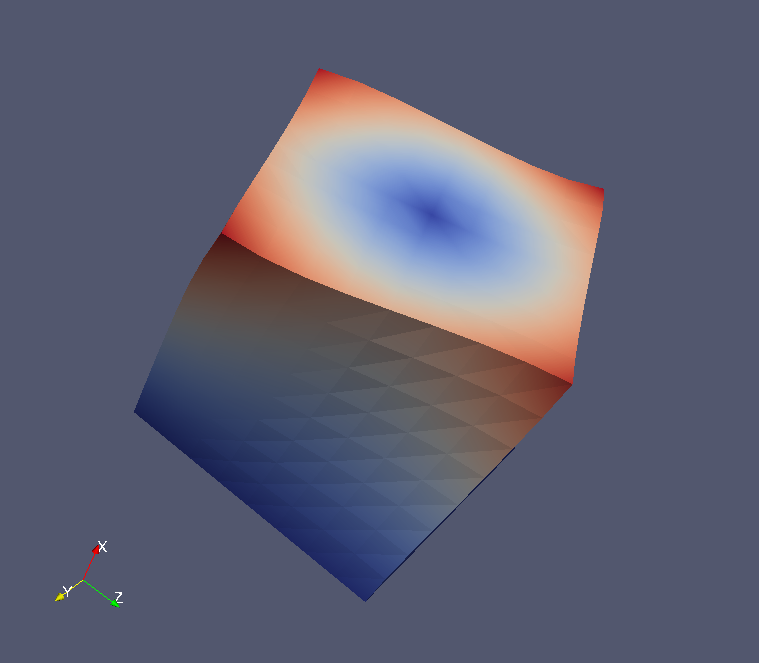
\includegraphics[width=\twofigsfull]{chapters/narayanan/images/png/release_000.png}
            }
            \subfloat[$t = 0.1$ s]{
              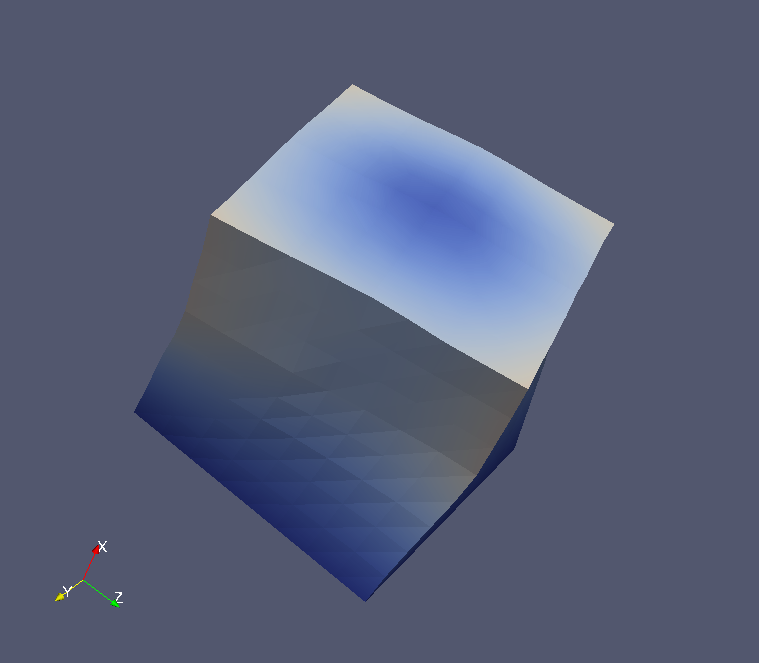
\includegraphics[width=\twofigsfull]{chapters/narayanan/images/png/release_100.png}
            } \\
            \subfloat[$t = 0.2$ s]{
              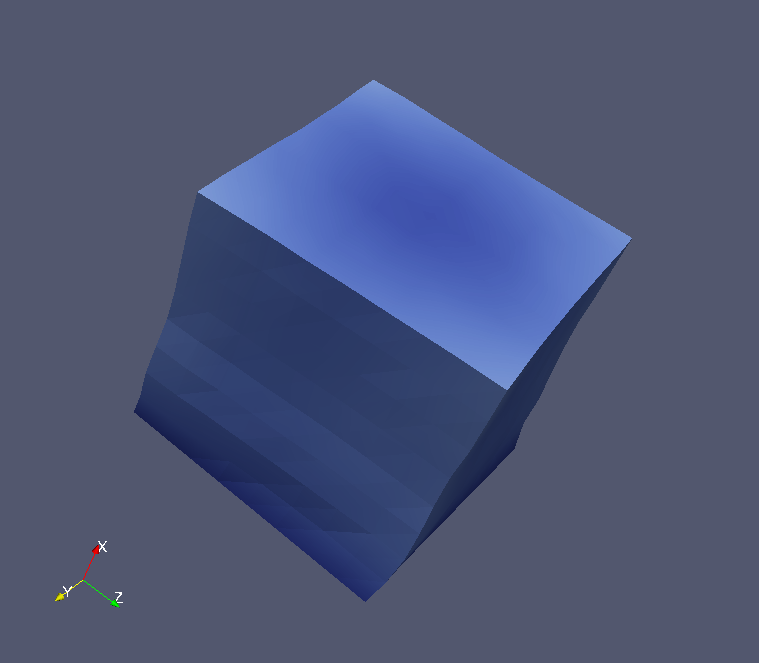
\includegraphics[width=\twofigsfull]{chapters/narayanan/images/png/release_200.png}
            }
            \subfloat[$t = 0.3$ s]{
              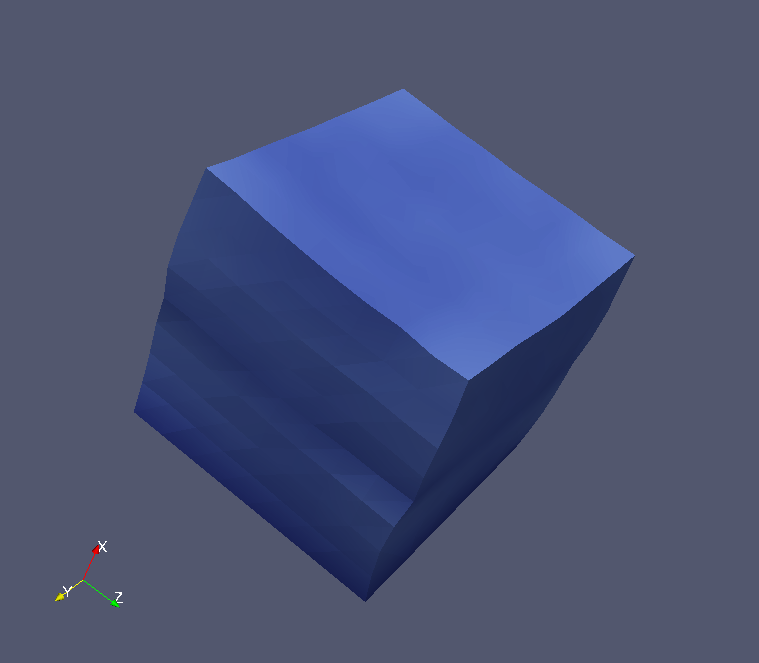
\includegraphics[width=\twofigsfull]{chapters/narayanan/images/png/release_300.png}
            } \\
            \subfloat[$t = 0.4$ s]{
              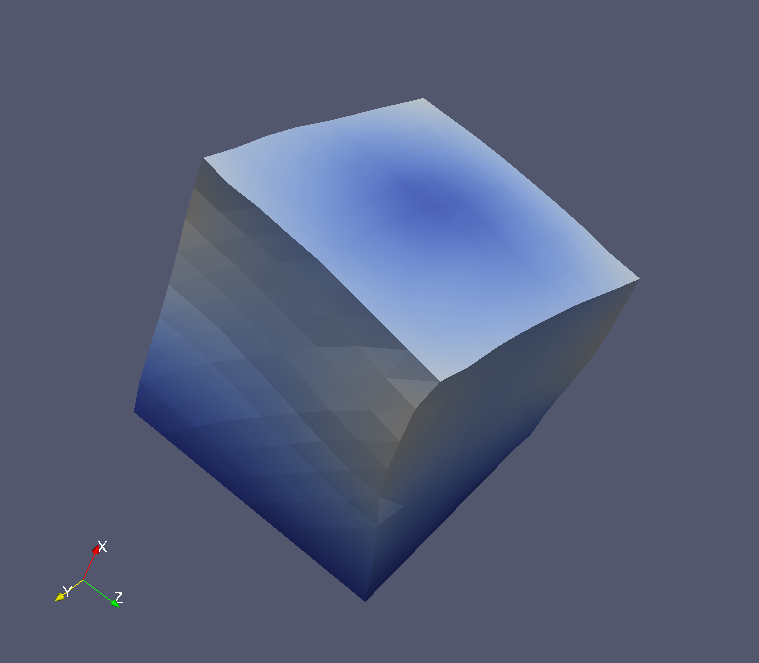
\includegraphics[width=\twofigsfull]{chapters/narayanan/images/png/release_400.png}
            }
            \subfloat[$t = 0.5$ s]{
              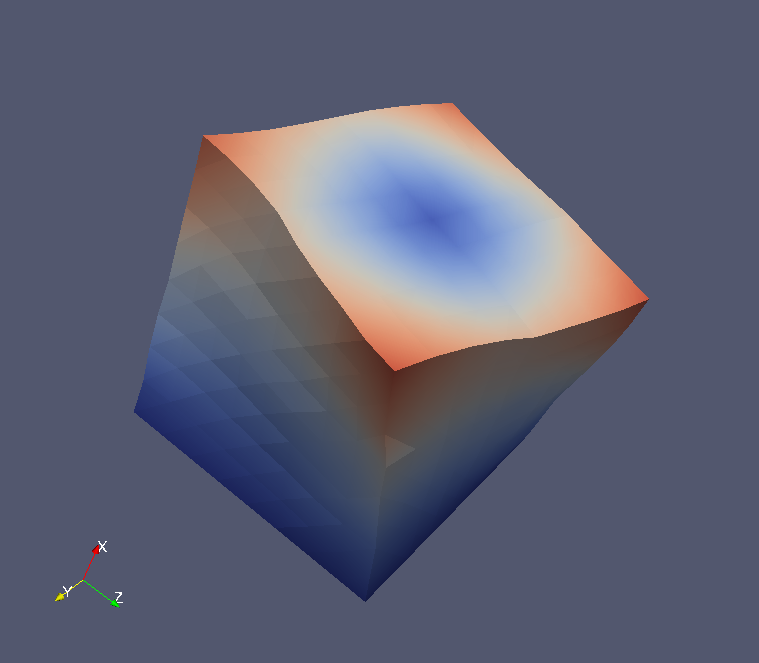
\includegraphics[width=\twofigsfull]{chapters/narayanan/images/png/release_500.png}
            }
}
\end{figure}

\begin{figure}
  \centering
  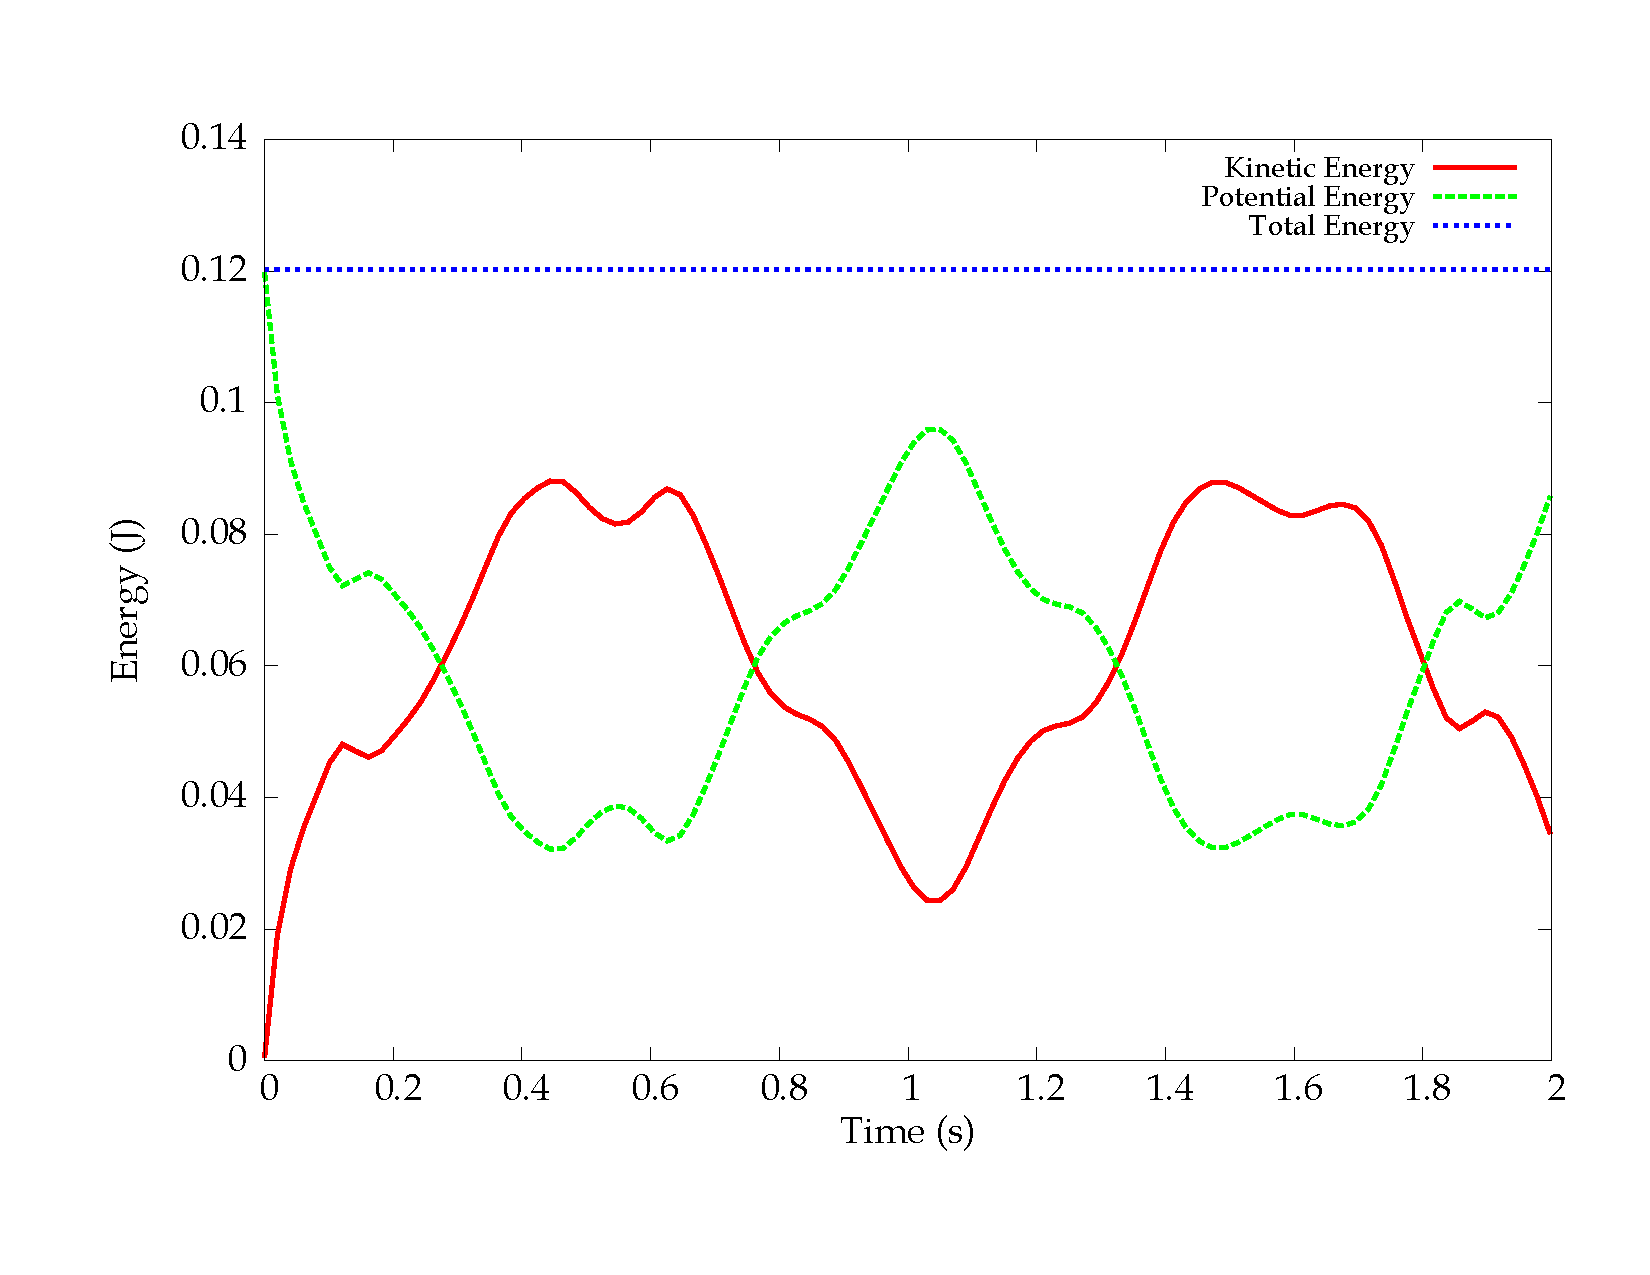
\includegraphics[width=\largefig]{chapters/narayanan/images/pdf/energies.pdf}
  \caption{Over the course of the computation, the energy in the body
    is converted between potential and kinetic energy, but the total
    remains constant.}
  \label{fig:narayanan:energies}
\end{figure}

\subsection{A hyperelastic dolphin tumbling through a ``flow''}

In this final example, we aim to crudely simulate the motion of a
dolphin under a flow field. The dolphin is assumed to be made out of a
Mooney--Rivlin material ($c_{1} = 6.169$~N/m$^2$, $c_{2} =
10.15$~N/m$^2$), and the flow field is simply modeled by a uniform
traction force $\bT = (0.05, 0)$~N acting everywhere on the surface of
the dolphin, pushing it to the right.

This example is constructed to exhibit some additional features of
\twist. For one, \twist{} is capable of performing dynamic calculations
under entirely Neumann boundary conditions. In addition, this
calculation points out that the framework can seamlessly handle
problems in two dimensions as well.

The problem is specified in the user-created class \emp{FishyFlow}
derived from \emp{Hyperelasticity}. There is nothing new to note in
the code listing for this problem (Figure~\ref{code:narayanan:%
fishyflow}), other than the fact that we now specify Neumann boundary
conditions. The specification listing is not very long because
\twist{} assumes meaningful default values for unspecified
information.

\begin{figure}
\bwfig
\begin{python}
class FishyFlow(Hyperelasticity):

    def mesh(self):
        mesh = Mesh("dolphin.xml.gz")
        return mesh

    def end_time(self):
        return 10.0

    def time_step(self):
        return 0.1

    def neumann_conditions(self):
        flow_push = Expression(("force", "0.0"), force=0.05)
        return [flow_push]

    def neumann_boundaries(self):
        everywhere = "on_boundary"
        return [everywhere]

    def material_model(self):

        material = MooneyRivlin([6.169, 10.15])
        return material
\end{python}
\caption{Problem definition: A hyperelastic dolphin being pushed to
  the right.}
\label{code:narayanan:fishyflow}
\end{figure}

To demonstrate one final piece of functionality of \twist, we don't
solve the problem in the same manner as we did the first two examples;
that is, we do not instantiate an object of class \emp{FishyFlow} and
call its \emp{solve} method. Instead, we set up our own time loop
and manually step through time using the \emp{step} method. This is
shown in Figure~\ref{code:narayanan:manualstep}.

\begin{figure}
\bwfig
\begin{python}
problem = FishyFlow()

dt = problem.time_step()
T = problem.end_time()

t = dt
while t <= T:
    problem.step(dt)
    problem.update()
    t = t + dt
\end{python}
\caption{Stepping through time in an external time loop. \emp{step}
  steps the problem forward by one time step, and \emp{update}
  updates the values of all time-dependent variables to the current time.}
\label{code:narayanan:manualstep}
\end{figure}

The advantage of solving the problem in this manner is that, now, one
has more control over calculations in \twist{}. For example, rather
than just fixing a traction force on the surface of the dolphin to
mimic the effect of flow field, one can instead solve at each time
step an actual flow field and use it to correctly drive the solid
mechanics. This functionality of \twist{} is used in a following
chapter on adaptive methods for fluid--structure interaction
(\ref{chap:selim}). In that work, the fluid--structure problem is
solved using a staggered approach with the solid mechanics equation
being solved by \twist. An external time loop similar to the one in
Figure~\ref{code:narayanan:manualstep} is set up to individually step
through the fluid problem, the solid problem and a mesh equation; a
process which is iterated until convergence is reached at each time
step. This process involves the systematic transfer of relevant
information (such as fluid loading) from other problems to \twist.

But returning to our current example,
Figure~\ref{fig:narayanan:tumblingdolphin} shows time snapshots of the
motion of the dolphin over the course of the computation. Notice that
the fish deforms elastically as it tumbles toward the right.

\begin{figure}
\bwfig
  \ffigbox{\caption{The motion of a hyperelastic dolphin being forced to the
      right. Careful observation of the tail fin shows deformation of
      the dolphin in addition to its overall motion toward the right.
      \label{fig:narayanan:tumblingdolphin}}}{}
  \ffigbox{}
          {
            \subfloat[$t = 0.0$ s]{
              
\includegraphics[width=\threefigsfull]{chapters/narayanan/images/png/dolphin_000.png}
            } \subfloat[$t = 0.125$ s]{
              
\includegraphics[width=\threefigsfull]{chapters/narayanan/images/png/dolphin_001.png}
            } \subfloat[$t = 0.250$ s]{
              
\includegraphics[width=\threefigsfull]{chapters/narayanan/images/png/dolphin_002.png}
            }\\ \subfloat[$t = 0.375$ s]{
              
\includegraphics[width=\threefigsfull]{chapters/narayanan/images/png/dolphin_003.png}
            } \subfloat[$t = 0.500$ s]{
              
\includegraphics[width=\threefigsfull]{chapters/narayanan/images/png/dolphin_004.png}
            } \subfloat[$t = 0.625$ s]{
              
\includegraphics[width=\threefigsfull]{chapters/narayanan/images/png/dolphin_005.png}
            }\\ \subfloat[$t = 0.750$ s]{
              
\includegraphics[width=\threefigsfull]{chapters/narayanan/images/png/dolphin_006.png}
            } \subfloat[$t = 0.875$ s]{
              
\includegraphics[width=\threefigsfull]{chapters/narayanan/images/png/dolphin_007.png}
            } \subfloat[$t = 1.000$ s]{
              
\includegraphics[width=\threefigsfull]{chapters/narayanan/images/png/dolphin_008.png}
            }
}
\end{figure}

\section{Conclusions}

This chapter presented an overview of \twist, an automated
computational framework for nonlinear elasticity. Beginning with
elements of classical nonlinear elasticity theory to motivate its
design, the discourse took a closer look at the algorithms underlying
\twist's implementation. The chapter concluded with some examples,
offering a tutorial-like description of how the framework can be used
in practice to solve problems.

The discussion aimed to highlight a central feature of \twist: the
ease with which different material models can be defined and
used. This feature makes \twist{} immediately applicable to a number
of real-world problems in engineering, especially those pertaining to
polymer and biological tissue mechanics.

\twist{} is a collaboratively developed open source project (released
under the GNU GPL) that is freely available from its source repository
at \url{https://launchpad.net/cbc.solve/}. Its only dependency is a
working FEniCS installation. \twist{} is released with the goal that
it will allow users to easily solve problems in nonlinear elasticity
as part of answering specific questions through computational
modeling. Everyone is encouraged to fetch and try it. Users are also
encouraged to modify the code to better suit their own purposes, and
contribute changes that they think are useful to the community. Along
these lines, some possible ideas for extending the framework include:
%%
\begin{itemize}
\item Implementing other specific material models
\item Allowing for bodies composed of multiple materials
\item Support for (nearly) incompressible materials
\item Support for anisotropic materials
\item Support for viscoelastic materials
\item Goal-oriented adaptivity
\end{itemize}
%%
Contributions toward these (or other useful) extensions are
welcome.
\enlargethispage{12pt}

\processqueries
\endgroup
